\documentclass[12pt,a4paper]{article}
\usepackage[T1]{fontenc}
\usepackage[utf8]{inputenc}
\usepackage{mathptmx}
\renewcommand{\figurename}{Figura}
\renewcommand{\tablename}{Tabela}
\usepackage[a4paper,left=3cm,right=3cm,top=2.5cm,bottom=2.5cm]{geometry}
\usepackage{amsmath,amssymb,amsthm}
\usepackage{graphicx}
\usepackage{booktabs}
\usepackage{algorithm}
\usepackage{algpseudocode}
\usepackage{tikz}
\usepackage[square,authoryear]{natbib}
\usepackage[colorlinks=true,linkcolor=black,citecolor=black,urlcolor=black]{hyperref}
\usepackage{url}
\usepackage{caption}
\captionsetup{font=small,labelfont=bf,labelsep=period,justification=centering}
\usetikzlibrary{positioning,arrows.meta}

\setlength{\parindent}{1.0cm}
\setlength{\parskip}{0pt}
\renewcommand{\baselinestretch}{1.0}

% títulos de seção no estilo SBC (negrito, sem serifa especial)
\makeatletter
\renewcommand{\section}{\@startsection{section}{1}{0pt}{-14pt plus -2pt minus -1pt}{6pt}{\normalfont\large\bfseries}}
\renewcommand{\subsection}{\@startsection{subsection}{2}{0pt}{-10pt plus -2pt minus -1pt}{4pt}{\normalfont\normalsize\bfseries}}
\makeatother

% resumo e abstract no estilo SBC (itálico, recuado)
\newenvironment{resumobloco}[1]
  {\begin{list}{}{\setlength{\leftmargin}{0.8cm}\setlength{\rightmargin}{0.8cm}\setlength{\itemindent}{0pt}\setlength{\listparindent}{0pt}}
   \item[]\small\itshape\textbf{#1.}\ }
  {\end{list}}

\theoremstyle{plain}
\newtheorem{lema}{Lema}
\newtheorem{teorema}{Teorema}
\theoremstyle{definition}
\newtheorem*{prova}{Demonstração}

% citações no formato do Trabalho 1: [Autor et al. 2002]
\renewcommand{\cite}{\citep}
\bibpunct[, ]{[}{]}{;}{a}{}{,}
\algrenewcommand\algorithmicrequire{\textbf{Entrada:}}
\algrenewcommand\algorithmicensure{\textbf{Saída:}}
\algrenewcommand\algorithmicif{\textbf{se}}
\algrenewcommand\algorithmicthen{\textbf{então}}
\algrenewcommand\algorithmicfor{\textbf{para}}
\algrenewcommand\algorithmicdo{\textbf{faça}}
\algrenewcommand\algorithmicreturn{\textbf{devolva}}
\algrenewcommand\algorithmicwhile{\textbf{enquanto}}
\algrenewcommand\algorithmicelse{\textbf{senão}}
\algrenewcommand\algorithmicend{\textbf{fim}}
\algrenewcommand\algorithmicforall{\textbf{para todo}}
\algrenewtext{EndIf}{\algorithmicend\ \algorithmicif}
\algrenewtext{EndFor}{\algorithmicend\ \algorithmicfor}
\algrenewtext{EndWhile}{\algorithmicend\ \algorithmicwhile}
\algrenewtext{EndProcedure}{\algorithmicend\ \algorithmicprocedure}
\renewcommand{\algorithmicprocedure}{\textbf{procedimento}}
\floatname{algorithm}{Algoritmo}

\begin{document}
\begin{center}
{\Large\bfseries Corte Máximo: Algoritmos Exatos por Branch-and-Bound\\ e Programação Dinâmica sobre a Largura de Caminho}\\[10pt]
{\bfseries Eduardo Marinho$^1$, Marcos Fontes$^1$}\\[6pt]
$^1$Centro de Ciências Exatas e da Terra\\
Departamento de Informática e Matemática Aplicada (DIMAp)\\
Universidade Federal do Rio Grande do Norte (UFRN) -- Natal, RN -- Brasil\\
DIM0605 -- Projeto e Análise de Algoritmos -- Prof.\ Sílvia Maia\\
Novembro de 2026
\end{center}
\vspace{6pt}
\begin{resumobloco}{Abstract}
This paper presents two exact algorithms for the Maximum Cut problem: a Branch-and-Bound, started from the heuristic of our previous work, and a dynamic program that sweeps the graph keeping only a small ``frontier'' of active vertices. Both are proved correct and were checked against brute force on 3,000 small graphs. On 12 instances with 100 to 100,002 vertices and a 15-minute limit per algorithm, the dynamic program found the optimum of 7 instances, including two toroidal grids of about 100,000 vertices (0.6 s and 9.2 s). Branch-and-Bound proved optimality for a single 100-vertex instance, because its upper bound is loose. With the optima, the previous heuristic reaches 77--79\% of the optimum on toroidal grids and 83--96\% on small sparse random graphs.
\end{resumobloco}
\vspace{8pt}
\begin{resumobloco}{Resumo}
Este trabalho apresenta dois algoritmos exatos para o problema do Corte Máximo: um Branch-and-Bound, iniciado com a heurística do trabalho anterior, e uma programação dinâmica que varre o grafo guardando apenas uma pequena ``fronteira'' de vértices ativos. Ambos têm prova de correção e foram conferidos contra força bruta em 3\,000 grafos pequenos. Em 12 instâncias de 100 a 100\,002 vértices, com limite de 15 minutos por algoritmo, a programação dinâmica calculou o ótimo de 7, inclusive duas grades toroidais de cerca de 100 mil vértices (0,6\,s e 9,2\,s). O Branch-and-Bound provou a otimalidade de uma única instância de 100 vértices, porque seu limite superior é folgado. Com os ótimos, a heurística do trabalho anterior obtém de 77\% a 79\% do ótimo nas grades toroidais e de 83\% a 96\% em grafos aleatórios esparsos pequenos.
\end{resumobloco}
\vspace{4pt}
\section{Introdução}

O problema do Corte Máximo (\emph{Max-Cut}) pede para dividir os vértices de um grafo em dois grupos de modo que o peso das arestas que ligam um grupo ao outro seja o maior possível. No Trabalho~1 usamos uma heurística simples (gulosa, com busca local) que resolve grafos de 100 mil vértices em milissegundos, mas que não garante o melhor resultado: nos grafos toroidais com pesos $\pm1$ do G-set ela ficou em torno de 80\% do melhor valor conhecido. Esse valor de referência vem de metaheurísticas \cite{Benlic and Hao 2013}, e não de uma prova de otimalidade, então não sabíamos o quanto da diferença era culpa da heurística.

Neste trabalho fazemos o contrário: usamos algoritmos \emph{exatos}, que devolvem o ótimo e provam que ele é o ótimo, ao custo de tempo exponencial no pior caso. Implementamos dois, de técnicas diferentes: um \emph{Branch-and-Bound} (explora as possibilidades e descarta as que não podem ser as melhores) e uma \emph{programação dinâmica} (varre o grafo mantendo na memória só o que ainda importa). Os dois foram conferidos contra força bruta em 3\,000 grafos pequenos.

Em vez de muitas instâncias pequenas, testamos 12 instâncias de tamanho significativo (de 100 a 100\,002 vértices), com até 15 minutos por algoritmo em cada uma. Em algumas, o ótimo é calculado e comparado com a heurística; em outras, o Branch-and-Bound trabalha até o limite de tempo e devolve a melhor solução que achou. Um aviso: um algoritmo exato escrito do zero não resolve as instâncias do G-set do Trabalho~1, e a literatura que resolve esses tamanhos usa ferramentas bem mais sofisticadas \cite{Liers et al. 2004, Rendl et al. 2010}. Por isso as instâncias misturam grafos aleatórios pequenos, grades toroidais estreitas (que chegam a 100 mil vértices por terem estrutura favorável) e instâncias difíceis, incluindo duas do G-set.

O texto segue a ordem pedida: problema e complexidade (Seção~2), estado da arte (Seção~3), técnicas escolhidas (Seção~4), algoritmos com prova de correção e análise de custo (Seção~5), instâncias e metodologia (Seção~6), resultados (Seção~7) e conclusão (Seção~8).


\section{Descrição do Problema}

Imagine dividir uma turma em dois times. Cada par de pessoas tem um número, o \emph{peso}: positivo se queremos separar os dois (rivalidade), negativo se preferimos que fiquem juntos. O objetivo é escolher os times de modo que a soma dos pesos dos pares \emph{separados} seja a maior possível.

Formalmente, temos um grafo não direcionado $G=(V,E)$ com $n$ vértices e $m$ arestas, e cada aresta $uv$ tem um peso inteiro $w_{uv}$. Uma partição atribui a cada vértice o lado 0 ou 1, e o valor do corte é a soma dos pesos das arestas cujas pontas ficam em lados diferentes. Queremos a partição de maior valor, $\mathrm{OPT}$. A notação é a mesma do Trabalho~1: $N(v)$ é a vizinhança de $v$ e $\Delta$ é o grau máximo.

\subsection{Complexidade}

O problema é NP-difícil \cite{Karp 1972, Garey et al. 1976}: não se conhece, e não se espera, um algoritmo que seja rápido em todos os casos. A forma mais direta de resolvê-lo é testar todas as divisões possíveis, $2^{n-1}$ delas (com $n=100$ são cerca de $10^{30}$, inviável). O melhor limite teórico conhecido para o caso geral é de ordem $1{,}73^n$ \cite{Williams 2005}, que ainda é exponencial e usa muita memória. Na prática, o que ajuda é a \emph{estrutura} do grafo: em grafos planares o problema tem solução rápida \cite{Hadlock 1975}, e em grafos que podem ser ``varridos'' com uma frente de largura $w$ ele se resolve em tempo proporcional a $2^{w}$ \cite{Arnborg et al. 1991, Bodlaender 1993}, o que é rápido se $w$ for pequeno. Esse é o caso das nossas grades toroidais estreitas, e é a ideia do segundo algoritmo.

\section{Estado da Arte em Algoritmos Exatos}

Os métodos exatos usados na prática para o Max-Cut se dividem em três famílias.

\paragraph{Branch-and-cut (programação linear).} Transforma o problema em um problema de programação linear e vai acrescentando restrições (desigualdades) que cortam soluções impossíveis. Foi aplicado a estados fundamentais de vidros de spin e ao projeto de circuitos \cite{Barahona et al. 1988}, e \citet{Liers et al. 2004} descrevem seu uso em casos difíceis. \citet{Liers et al. 2003} resolveram grafos aleatórios regulares de grau 4 e 6 com até 1\,280 vértices, classe parecida com os nossos aleatórios esparsos (que têm grau médio 4). É, em geral, o método mais indicado para grafos esparsos.

\paragraph{Branch-and-bound semidefinido.} Usa uma relaxação mais forte (programação semidefinida) para calcular os limites. O \emph{Biq Mac} \cite{Rendl et al. 2010} resolve qualquer instância com até 100 vértices, qualquer que seja a densidade, e é a referência para grafos densos; os autores observam que, para grafos esparsos, os métodos de programação linear podem ser melhores. \citet{Krislock et al. 2014} melhoraram o cálculo desses limites.

\paragraph{Aproveitar a estrutura do grafo.} Para grafos de largura de caminho ou de árvore pequena, a programação dinâmica é exata e custa $O(2^{w}\cdot\mathrm{poly}(n))$ \cite{Arnborg et al. 1991, Bodlaender 1993}. A largura de caminho é a menor ``frente de varredura'' que se consegue em alguma ordem dos vértices \cite{Kinnersley 1992}, o que permite implementar a ideia como um simples percurso, como fazemos na Seção~5.2.

Nossos algoritmos são versões simples dessas ideias: o Branch-and-Bound usa um limite bem mais barato (e mais fraco) que os das duas primeiras famílias, e a programação dinâmica é a versão mais básica da terceira. Não esperamos competir com o \emph{Biq Mac} nem com os resolvedores de branch-and-cut, e a comparação da Seção~7 deve ser lida com esse cuidado.

\section{Técnicas Escolhidas}

\paragraph{Branch-and-Bound: tentar e podar.} É como percorrer um labirinto de decisões. Escolhemos o lado de um vértice de cada vez (duas opções), formando uma árvore de possibilidades. Antes de seguir por um ramo, calculamos um \emph{teto}: o melhor corte que ainda seria possível nesse ramo, na melhor das hipóteses. Se o teto não supera a melhor solução já encontrada, o ramo inteiro é descartado (podado), sem precisar visitá-lo. Quanto mais justo o teto, mais se poda. Começamos com a heurística do Trabalho~1 como ``melhor solução já vista'', o que liga os dois trabalhos: uma heurística boa poda mais desde o início.

\paragraph{Programação dinâmica: lembrar só o necessário.} É como ler um livro de capítulo em capítulo anotando num quadro só o que ainda será citado adiante. Processamos os vértices em uma ordem fixa. O \emph{quadro} é a \emph{fronteira}: os vértices já processados que ainda têm vizinhos por processar. Para cada combinação de lados dos vértices do quadro, guardamos o melhor valor obtido até ali. Quando um vértice perde o último vizinho pendente, ele sai do quadro, e ficamos com o melhor de seus dois lados. A Figura~\ref{fig:fronteira} mostra o percurso. O custo cresce com o tamanho do quadro (a largura $w$), e não com $n$.

As duas técnicas se complementam. O Branch-and-Bound funciona em qualquer grafo, mas o tempo explode com $n$ mesmo em grafos esparsos. A programação dinâmica depende de o grafo ter uma frente de varredura pequena, mas, quando tem, resolve instâncias com dezenas de milhares de vértices.

\begin{figure}[ht]
\centering
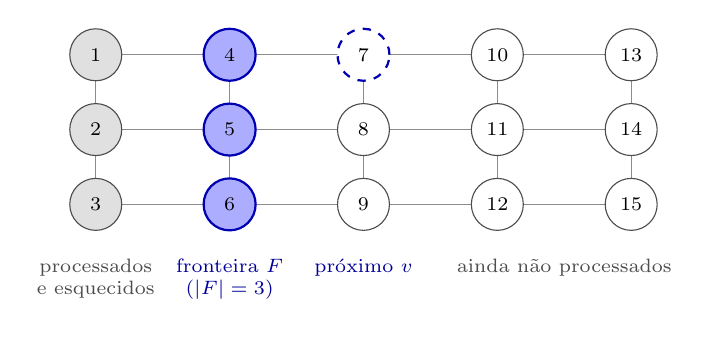
\begin{tikzpicture}[x=1.7cm,y=-0.95cm,
  vtx/.style={circle,draw=black!70,minimum size=0.66cm,inner sep=0pt,font=\scriptsize},
  proc/.style={vtx,fill=black!12},
  fron/.style={vtx,fill=blue!32,draw=blue!70!black,thick},
  prox/.style={vtx,fill=white,draw=blue!70!black,thick,dashed},
  nao/.style={vtx,fill=white},
  aresta/.style={draw=black!45}]
  \foreach \c in {1,...,5}{\foreach \r in {1,2,3}{
    \pgfmathtruncatemacro{\id}{(\c-1)*3+\r}
    \coordinate (p\c\r) at (\c,\r);
  }}
  \foreach \c in {1,...,5}{\foreach \r in {1,2,3}{
    \pgfmathtruncatemacro{\cc}{\c+1}\pgfmathtruncatemacro{\rr}{\r+1}
    \ifnum\c<5 \draw[aresta] (p\c\r) -- (p\cc\r); \fi
    \ifnum\r<3 \draw[aresta] (p\c\r) -- (p\c\rr); \fi
  }}
  \foreach \c/\sty in {1/proc,2/fron,3/nao,4/nao,5/nao}{\foreach \r in {1,2,3}{
    \pgfmathtruncatemacro{\id}{(\c-1)*3+\r}
    \ifnum\c=3\ifnum\r=1 \node[prox] at (p\c\r) {\id}; \else \node[nao] at (p\c\r) {\id}; \fi
    \else \node[\sty] at (p\c\r) {\id}; \fi
  }}
  \node[anchor=north,align=center,font=\scriptsize,text=black!70] at (1,3.6) {processados\\e esquecidos};
  \node[anchor=north,align=center,font=\scriptsize,text=blue!60!black] at (2,3.6) {fronteira $F$\\($|F|=3$)};
  \node[anchor=north,align=center,font=\scriptsize,text=blue!60!black] at (3,3.6) {próximo $v$};
  \node[anchor=north,align=center,font=\scriptsize,text=black!70] at (4.5,3.6) {ainda não processados};
\end{tikzpicture}
\caption{Percurso da programação dinâmica em uma grade $3\times5$ numerada por colunas. Os vértices 1 a 3 já saíram da fronteira (todos os seus vizinhos foram processados); os vértices 4 a 6 formam a fronteira $F$, porque cada um ainda tem vizinho na coluna seguinte. Ao inserir o vértice 7, a tabela tem $2^{|F|+1}=16$ entradas.}\label{fig:fronteira}
\end{figure}


\section{Algoritmos Implementados}

\subsection{Algoritmo 1: Branch-and-Bound}

\paragraph{Como funciona.} Os vértices são decididos um a um, em uma ordem escolhida de forma gulosa: o próximo é sempre o que tem mais peso ligado aos vértices já decididos. Assim as arestas ficam ``resolvidas'' cedo, e o teto fica justo mais rápido. Para cada vértice, tentamos primeiro o lado que corta mais peso.

\paragraph{O teto.} Em um ponto da busca, parte dos vértices já tem lado. O teto soma três coisas: (i) o valor das arestas já resolvidas que estão cortadas; (ii) para cada vértice ainda livre, o máximo entre os dois lados do que ele ganharia com as arestas para vértices já decididos (é o $\max\{c_0(v),c_1(v)\}$ abaixo, em que $c_s(v)$ é o peso das arestas de $v$ para decididos do lado $s$); e (iii) para cada aresta entre dois vértices livres, o seu peso se for positivo (na melhor das hipóteses ela é cortada). Em fórmula,
\begin{equation}\label{eq:ub}
  \mathrm{teto}=\mathrm{corte\ atual}+\sum_{v\ \text{livre}}\max\{c_0(v),c_1(v)\}+\sum_{\substack{uv\in E\\ u,v\ \text{livres}}}\max\{w_{uv},0\}.
\end{equation}
Esse valor é atualizado de forma incremental, mexendo só no vértice decidido e em seus vizinhos. Um detalhe: como trocar os dois lados de todos os vértices de uma componente conexa não altera o corte, o primeiro vértice de cada componente é fixado no lado 0, o que corta a busca pela metade por componente.

\begin{algorithm}[ht]
\caption{Branch-and-Bound}\label{alg:bb}
\begin{algorithmic}[1]
\Require grafo $G=(V,E,w)$, tempo máximo $T$
\Ensure a melhor partição encontrada (é ótima se a busca terminar antes de $T$)
\State $s^*\gets$ heurística do Trabalho 1; \quad $\mathit{melhor}\gets$ valor de $s^*$
\State definir a ordem dos vértices e calcular o teto inicial
\Procedure{Busca}{$i$}
  \If{$\mathrm{teto}\le\mathit{melhor}$} \State \textbf{retornar} \Comment{poda: este ramo não pode vencer}
  \EndIf
  \If{todos os vértices decididos} \State $\mathit{melhor}\gets$ corte atual; \quad $s^*\gets$ partição atual; \quad \textbf{retornar}
  \EndIf
  \State $v\gets$ $i$-ésimo vértice da ordem
  \For{cada lado $s\in\{0,1\}$ (primeiro o que corta mais; pular $s=1$ se $v$ abre componente)}
    \State decidir $v$ no lado $s$; \quad \Call{Busca}{$i+1$}; \quad desfazer a decisão
  \EndFor
\EndProcedure
\State \Call{Busca}{$1$}; \quad \textbf{devolva} $s^*$
\end{algorithmic}
\end{algorithm}

\paragraph{Por que está correto.} O ponto-chave é que o teto nunca subestima.

\begin{lema}\label{lema:ub}
Qualquer forma de completar uma solução parcial tem corte menor ou igual ao teto \eqref{eq:ub}.
\end{lema}
\begin{prova}
As arestas já resolvidas contribuem exatamente o ``corte atual''. Cada vértice livre só consegue cortar as arestas para decididos do lado oposto ao seu, o que vale no máximo $\max\{c_0(v),c_1(v)\}$. Cada aresta entre dois livres contribui $w_{uv}$ ou $0$, no máximo $\max\{w_{uv},0\}$. Somando, o teto cobre todos os casos. \qed
\end{prova}

\begin{teorema}[Correção]\label{teo:bb}
Se a busca termina antes do limite de tempo, a partição devolvida é ótima.
\end{teorema}
\begin{prova}
O valor $\mathit{melhor}$ sempre corresponde a uma partição válida. Suponha que existisse uma partição melhor que a devolvida; podemos supor que ela respeita a regra de fixar o primeiro vértice de cada componente no lado 0, pois trocar os lados de uma componente inteira não muda o corte. Em todo ponto do caminho que leva a essa partição, o teto é pelo menos o valor dela (Lema~\ref{lema:ub}), que é maior que $\mathit{melhor}$; logo nenhum ramo desse caminho é podado, a busca chega à partição e atualiza $\mathit{melhor}$, uma contradição. \qed
\end{prova}

\paragraph{Custo.} Cada decisão custa $O(\text{grau do vértice})$, e a árvore tem no máximo $2^{n}$ folhas, então o pior caso é $O(2^{n}\,\Delta)$ em tempo e $O(n+m)$ em memória. Não há garantia melhor: se o teto for folgado, quase nada é podado. É exatamente o que acontece nos grafos esparsos (Seção~7).

\subsection{Algoritmo 2: Programação dinâmica sobre a fronteira}

\paragraph{Como funciona.} Fixamos uma ordem $v_1,\dots,v_n$ e processamos os vértices um a um. A \emph{fronteira} $F$ é o conjunto dos vértices já processados que ainda têm vizinhos por processar. Guardamos uma tabela $f$ que, para cada combinação de lados dos vértices de $F$, dá o maior valor de corte, contando só as arestas entre vértices já processados. Cada passo tem duas fases (Figura~\ref{fig:passo}): o vértice novo entra, e os vértices que não têm mais vizinhos pendentes saem.

\begin{figure}[ht]
\centering
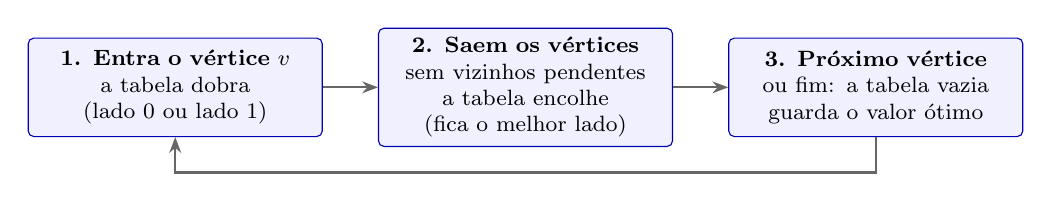
\begin{tikzpicture}[caixa/.style={draw=blue!70!black,fill=blue!6,rounded corners=2pt,align=center,font=\footnotesize,text width=3.5cm,minimum height=1.25cm},
  seta/.style={-{Stealth[length=2mm]},thick,draw=black!60}]
  \node[caixa] (a) {\textbf{1. Entra o vértice $v$}\\a tabela dobra\\(lado 0 ou lado 1)};
  \node[caixa,right=0.7cm of a] (b) {\textbf{2. Saem os vértices}\\sem vizinhos pendentes\\a tabela encolhe\\(fica o melhor lado)};
  \node[caixa,right=0.7cm of b] (c) {\textbf{3. Próximo vértice}\\ou fim: a tabela vazia\\guarda o valor ótimo};
  \draw[seta] (a)--(b); \draw[seta] (b)--(c);
  \draw[seta] (c.south) -- ++(0,-0.45) -| (a.south);
\end{tikzpicture}
\caption{Um passo da programação dinâmica.}\label{fig:passo}
\end{figure}

\begin{algorithm}[ht]
\caption{Programação dinâmica sobre a fronteira}\label{alg:dp}
\begin{algorithmic}[1]
\Require grafo $G=(V,E,w)$ e uma ordem $v_1,\dots,v_n$ dos vértices
\Ensure o valor ótimo e uma partição ótima
\State $F\gets$ lista vazia; \quad $f\gets$ tabela com uma única entrada, de valor $0$
\For{$t=1$ \textbf{até} $n$}
  \State $v\gets v_t$
  \ForAll{combinação $x$ de lados de $F$ \textbf{e} lado $s\in\{0,1\}$ para $v$} \Comment{se $F$ é vazia, só $s=0$}
    \State $h[x,s]\gets f[x]+{}$soma dos pesos das arestas de $v$ para vértices de $F$ que estão no lado oposto a $s$
  \EndFor
  \State $F\gets F\cup\{v\}$; \quad $f\gets h$ \Comment{agora a tabela cobre $F$ inclusive $v$}
  \ForAll{$u\in F$ sem vizinhos ainda não processados}
    \State trocar $f$ por $f'[y]=\max\{f[y,u{=}0],\,f[y,u{=}1]\}$, \textbf{guardando} qual lado de $u$ venceu
    \State remover $u$ de $F$
  \EndFor
\EndFor
\State \textbf{devolva} $f[\,]$ \Comment{$F$ ficou vazia: a única entrada é o valor ótimo}
\State recuperar a partição percorrendo os passos de trás para frente, lendo o lado que venceu em cada remoção
\end{algorithmic}
\end{algorithm}

\paragraph{Por que está correto.} A ideia é que a tabela sempre responde exatamente à pergunta: ``qual o melhor corte entre os vértices já processados, dado que a fronteira está nesta configuração?''

\begin{teorema}[Correção]\label{teo:dp}
Para qualquer ordem dos vértices, o Algoritmo~\ref{alg:dp} devolve o valor ótimo e uma partição que o atinge.
\end{teorema}
\begin{prova}
Por indução no número de vértices processados. No passo em que $v$ entra, os vizinhos de $v$ já processados estão todos na fronteira (cada um tem $v$ como vizinho pendente); logo as arestas novas só dependem dos lados da fronteira e do lado de $v$, e a soma da linha~5 as conta exatamente. Um vértice $u$ só sai quando todos os seus vizinhos já foram processados; assim, nenhuma aresta futura depende do lado de $u$, e escolher o melhor lado dele não descarta nenhuma solução. Ao final, a fronteira está vazia e a tabela guarda o máximo sobre todas as partições. A restrição $s=0$ para um vértice que abre uma componente não perde o ótimo, pelo mesmo argumento de simetria do Teorema~\ref{teo:bb}. A reconstrução desfaz as escolhas em ordem inversa, usando o lado que venceu em cada remoção. \qed
\end{prova}

\paragraph{Custo.} Seja $w$ o maior número de vértices que a tabela cobre em algum passo (a fronteira mais o vértice que entra). A tabela tem então até $2^{w}$ entradas. Cada vértice entra uma vez, e para cada entrada somamos as arestas para a fronteira; cada remoção percorre a tabela uma vez. O tempo total é $O(2^{w}(n+m))$. A memória é $O(2^{w})$ para a tabela, mais $O(n\,2^{w})$ \emph{bits} para guardar qual lado venceu em cada remoção (necessários para reconstruir a partição). Com a melhor ordem possível, $w-1$ é a largura de caminho do grafo \cite{Kinnersley 1992}; achar essa ordem é difícil, e usamos uma heurística.

\paragraph{Escolha da ordem.} A ordem é gulosa: em cada passo, entre os vértices vizinhos da fronteira, escolhemos o que deixa a fronteira menor (desempate pelo menor número de vizinhos pendentes e, depois, ao acaso). Repetimos a construção a partir de até 30 vértices iniciais diferentes e ficamos com a de menor $w$. Antes de alocar qualquer tabela, o programa calcula $w$ e a memória necessária e se recusa a executar se $w>26$ ou se passar de 2\,GB. Nas grades toroidais de lado curto $L$, o guloso acha $w=2L+1$ (Tabela~\ref{tab:principal}).

\section{Instâncias e Metodologia}\label{sec:instancias}

\subsection{Escolha das instâncias}

Usamos 12 instâncias, em três grupos (Tabela~\ref{tab:familias}). O grupo A tem grafos aleatórios esparsos ($m=2n$, grau médio 4, como a R100k do Trabalho~1), pequenos o bastante para o ótimo ser calculado. O grupo B tem grades toroidais com pesos $\pm1$ e lado curto $L$ pequeno: a largura da programação dinâmica é $2L+1$ e não depende do comprimento da grade, então o ótimo sai até com 100 mil vértices. O grupo C tem instâncias em que a programação dinâmica é inviável (largura de 41 ou mais): ali só roda o Branch-and-Bound, que devolve a melhor solução achada em 15 minutos. Duas delas, o G32 e o G57, vêm do Trabalho~1.

Não usamos o G-set inteiro porque, para essas instâncias, a melhor ordem que o guloso encontra tem fronteira de 41 no G32 e acima de 60 nas demais (a tabela teria pelo menos $2^{41}$ entradas, contra o limite prático de $2^{26}$). Isso não quer dizer que elas não possam ser resolvidas, só que estão fora do alcance do que implementamos.

\begin{table}[ht]\centering\footnotesize
\caption{Instâncias do experimento. $w$: menor largura de fronteira que o guloso encontrou (``$>$'': desistiu acima do valor indicado).}\label{tab:familias}
\begin{tabular}{llrcl}\hline
Grupo & Instância & $n$ & $w$ & Descrição\\\hline
A & \texttt{01\_ALE\_n100} & 100 & 21 & aleatória esparsa, pesos $+1$\\
A & \texttt{02\_ALE\_n120} & 120 & 26 & aleatória esparsa, pesos $+1$\\
A & \texttt{03\_PM1\_n120} & 120 & 26 & aleatória esparsa, pesos $\pm1$\\
B & \texttt{04\_TORO\_8x250} & 2\,000 & 17 & grade toroidal $8\times250$, pesos $\pm1$\\
B & \texttt{05\_TORO\_10x200} & 2\,000 & 21 & grade toroidal $10\times200$, pesos $\pm1$\\
B & \texttt{06\_TORO\_5x20000} & 100\,000 & 11 & grade toroidal $5\times20000$, pesos $\pm1$\\
B & \texttt{07\_TORO\_7x14286} & 100\,002 & 15 & grade toroidal $7\times14286$, pesos $\pm1$\\
C & \texttt{08\_ALE\_n200} & 200 & 42 & aleatória esparsa, pesos $+1$\\
C & \texttt{09\_PM1\_n500} & 500 & $>80$ & aleatória esparsa, pesos $\pm1$\\
C & \texttt{10\_TORO\_20x50} & 1\,000 & 41 & grade toroidal $20\times50$, pesos $\pm1$\\
C & \texttt{11\_G32} & 2\,000 & 41 & G-set (Trabalho 1), pesos $\pm1$\\
C & \texttt{12\_G57} & 5\,000 & $>60$ & G-set (Trabalho 1), pesos $\pm1$\\\hline
\end{tabular}
\end{table}

\subsection{Geradores}

Usamos o gerador do Trabalho~1 e um novo, \texttt{gerador\_t2.cpp}, com o mesmo formato de arquivo (\texttt{n m} e uma linha \texttt{u v peso} por aresta). Ele tem dois modos, ambos determinísticos para uma dada semente: \texttt{aleatorio n m semente pesos}, que sorteia $m$ arestas distintas (pesos todos $+1$ ou $\pm1$ com probabilidade $1/2$); e \texttt{toro L C semente}, que gera uma grade toroidal $L\times C$ (cada vértice com 4 vizinhos), com pesos $\pm1$ e rótulos embaralhados para que a estrutura de grade não apareça na numeração. Todas as instâncias geradas usam a semente 1.

\subsection{Plataforma e protocolo}

Os experimentos rodaram em um computador com processador Intel Core i5-9300H a 2,40\,GHz e 8\,GB de RAM, em execução \emph{single-thread}, sob Windows 11, com o compilador \texttt{g++} 15.1 e as opções \texttt{-std=c++17 -O2}. Os tempos são de relógio de parede e medem só o algoritmo, sem a leitura do arquivo. Cada instância foi executada uma única vez, com limite de 900\,s (15 minutos) \emph{por algoritmo}. Se o Branch-and-Bound estoura o limite, devolve a melhor solução encontrada e a otimalidade não é provada. A programação dinâmica roda com $w\le26$ e até 2\,GB de memória; ela não devolve solução parcial: ou termina com o ótimo, ou não executa. O Branch-and-Bound não roda para $n>5\,000$, o que afeta apenas as instâncias 06 e 07.

A heurística do Trabalho~1 está incorporada ao programa novo, mas a leitura agora ordena as listas de vizinhos, o que muda o desempate da ordenação por grau. É o mesmo algoritmo, mas não idêntico bit a bit: no G32 ele dá 1\,170 aqui contra 1\,154 no relatório anterior, e no G57, 2\,924 contra 2\,848. Neste relatório usamos sempre a versão incorporada.

\subsection{Validação}

Um programa de validação (\texttt{validacao.cpp}) gera 3\,000 grafos aleatórios com 1 a 16 vértices, densidades de 0 a 1 e quatro regimes de pesos (todos $+1$; $\pm1$; inteiros em $[-4,6]$, inclusive nulos; inteiros em $[1,9]$) e compara o ótimo obtido por força bruta com o dos dois algoritmos, recalculando também o corte das partições devolvidas. A força bruta é usada só como oráculo de teste. Essa validação foi feita durante o desenvolvimento, em um ambiente Linux com \texttt{g++} 13.3: 3\,000 casos, 0 falhas. Além disso, os ótimos das instâncias 01 a 07 obtidos nesse ambiente coincidem exatamente com os da máquina do experimento, e a partição final de cada execução é sempre reavaliada pelo programa.

\subsection{Reprodução}

O pacote entregue contém código, instâncias e scripts. A partir da pasta do projeto:
\begin{verbatim}
bash scripts/rodar_experimentos_longos.sh 900
python3 scripts/gerar_tabelas_figuras.py
./exato instancias_longas/04_TORO_8x250
\end{verbatim}
O primeiro comando roda as 12 instâncias (15 minutos por algoritmo), o segundo gera tabelas e figuras a partir do CSV, e o terceiro roda uma instância (\texttt{./exato} sem argumentos abre um menu). As instâncias estão em \texttt{instancias\_longas/} e podem ser recriadas com \texttt{scripts/gerar\_instancias\_longas.sh}.

\section{Resultados e Discussão}

A Tabela~\ref{tab:principal} traz o resultado de cada instância e da programação dinâmica; a Tabela~\ref{tab:bb} mostra o que o Branch-and-Bound fez em 15 minutos; as Figuras~\ref{fig:razao} e~\ref{fig:tempos} resumem a qualidade e o tempo. Todos os números vêm do arquivo \texttt{resultados.csv} do experimento, e onde os dois algoritmos terminaram os valores coincidiram.

\begin{table}[ht]\centering\footnotesize\setlength{\tabcolsep}{4pt}
\caption{Resultados nas 12 instâncias. Ótimo/melhor: ótimo provado (sem marca) ou melhor valor encontrado, sem prova de otimalidade ($^*$). Heur.: heurística do Trabalho~1. Razão: Heur./ótimo. DP: largura $w$, tempo e memória estimada (``---'': inviável, $w>26$).}\label{tab:principal}
\begin{tabular}{lrrrrcrrr}\hline
Instância & $n$ & $m$ & Ótimo/melhor & Heur. & Razão & $w$ & DP (s) & Mem. (MB) \\\hline
01\_ALE\_n100 & 100 & 200 & 168 & 158 & 0{,}940 & 21 & 0{,}173 & 26 \\
02\_ALE\_n120 & 120 & 240 & 204 & 196 & 0{,}961 & 26 & 5{,}139 & 845 \\
03\_PM1\_n120 & 120 & 240 & 83 & 69 & 0{,}831 & 26 & 5{,}147 & 845 \\
04\_TORO\_8x250 & 2000 & 4000 & 1406 & 1114 & 0{,}792 & 17 & 0{,}811 & 16 \\
05\_TORO\_10x200 & 2000 & 4000 & 1386 & 1080 & 0{,}779 & 21 & 12{,}9 & 265 \\
06\_TORO\_5x20000 & 100000 & 200000 & 69050 & 53738 & 0{,}778 & 11 & 0{,}632 & 12 \\
07\_TORO\_7x14286 & 100002 & 200004 & 69354 & 53570 & 0{,}772 & 15 & 9{,}195 & 195 \\
08\_ALE\_n200 & 200 & 400 & 322$^*$ & 316 & --- & --- & --- & --- \\
09\_PM1\_n500 & 500 & 1000 & 299$^*$ & 299 & --- & --- & --- & --- \\
10\_TORO\_20x50 & 1000 & 2000 & 528$^*$ & 516 & --- & --- & --- & --- \\
11\_G32 & 2000 & 4000 & 1170$^*$ & 1170 & --- & --- & --- & --- \\
12\_G57 & 5000 & 10000 & 2924$^*$ & 2924 & --- & --- & --- & --- \\
\hline\end{tabular}

\end{table}

\begin{table}[ht]\centering\footnotesize\setlength{\tabcolsep}{4pt}
\caption{Branch-and-Bound com limite de 900\,s. Situação: ótimo provado ou parou no limite. Nós: milhares de milhões de nós visitados. Limitante inicial: o teto \eqref{eq:ub} antes de qualquer decisão. Melhorias: quantas vezes a melhor solução encontrada melhorou.}\label{tab:bb}
\begin{tabular}{lrcrrrr}\hline
Instância & Valor & Situação & Tempo (s) & Nós ($10^9$) & Limitante inicial & Melhorias \\\hline
01\_ALE\_n100 & 168 & ótimo & 620 & 19{,}1 & 200 & 10 \\
02\_ALE\_n120 & 201 & limite & 900 & 32{,}1 & 240 & 5 \\
03\_PM1\_n120 & 75 & limite & 900 & 30{,}9 & 119 & 6 \\
04\_TORO\_8x250 & 1114 & limite & 900 & 32{,}9 & 2001 & 0 \\
05\_TORO\_10x200 & 1080 & limite & 900 & 31{,}3 & 2001 & 0 \\
06\_TORO\_5x20000 & \multicolumn{6}{c}{não executado ($n>5000$)} \\
07\_TORO\_7x14286 & \multicolumn{6}{c}{não executado ($n>5000$)} \\
08\_ALE\_n200 & 322 & limite & 900 & 35{,}9 & 400 & 6 \\
09\_PM1\_n500 & 299 & limite & 900 & 51{,}6 & 517 & 0 \\
10\_TORO\_20x50 & 528 & limite & 900 & 35{,}9 & 993 & 4 \\
11\_G32 & 1170 & limite & 900 & 34{,}4 & 2011 & 0 \\
12\_G57 & 2924 & limite & 900 & 34{,}5 & 4981 & 0 \\
\hline\end{tabular}

\end{table}

\begin{figure}[ht]
\centering
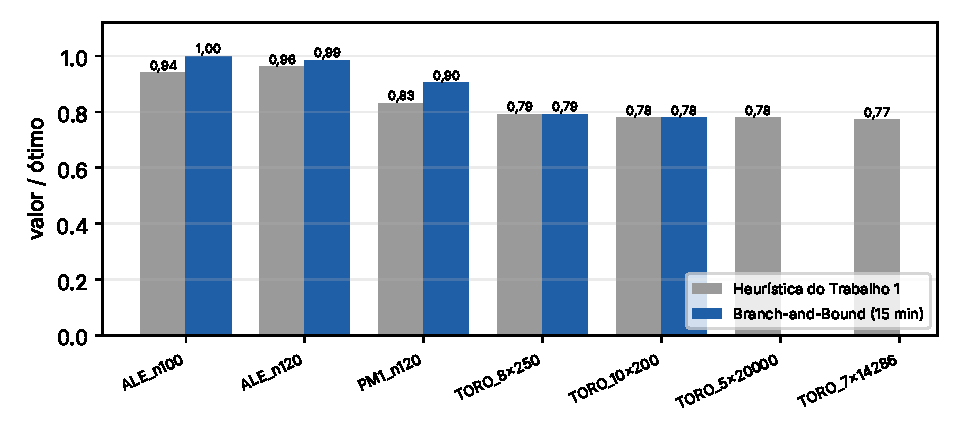
\includegraphics[width=0.92\textwidth]{fig_razao.pdf}
\caption{Valor obtido em relação ao ótimo nas instâncias em que a programação dinâmica calculou o ótimo: heurística do Trabalho~1 (cinza) e Branch-and-Bound com 15 minutos (azul). O Branch-and-Bound não roda nas instâncias de 100 mil vértices.}\label{fig:razao}
\end{figure}

\begin{figure}[ht]
\centering
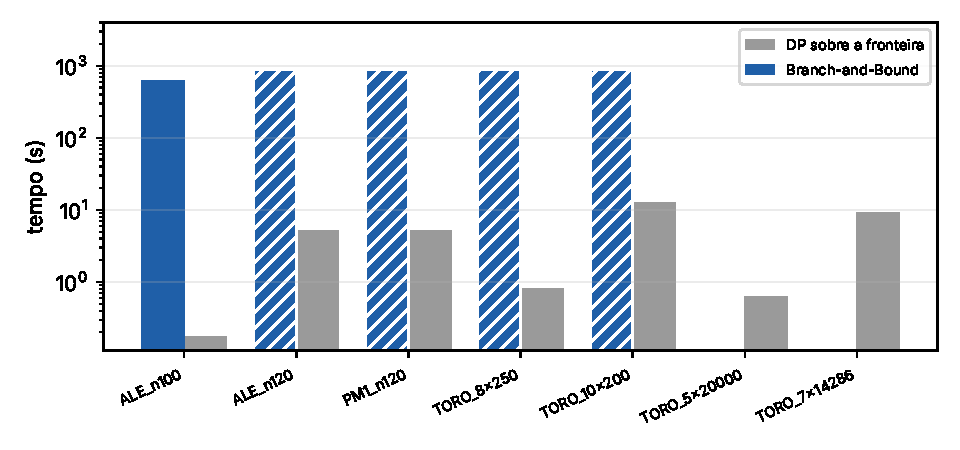
\includegraphics[width=0.92\textwidth]{fig_tempos.pdf}
\caption{Tempo do Branch-and-Bound (azul) e da programação dinâmica (cinza), em escala logarítmica. Barras hachuradas: o Branch-and-Bound parou no limite de 900\,s sem provar o ótimo.}\label{fig:tempos}
\end{figure}

\subsection{Programação dinâmica}

A programação dinâmica calculou o ótimo das 7 instâncias dos grupos A e B, inclusive as duas grades de cerca de 100 mil vértices, em 0,63\,s ($w=11$) e 9,2\,s ($w=15$). O tempo depende de $w$, e quase nada de $n$: cada 4 unidades a mais de largura multiplicam o tempo por cerca de 16 ($0{,}81$\,s com $w=17$ e $12{,}9$\,s com $w=21$, ambas com 2\,000 vértices), como previsto por $O(2^{w}(n+m))$. A memória acompanha: de 12\,MB ($w=11$) a 845\,MB ($w=26$, o limite da implementação). Nas instâncias do grupo C, a fronteira encontrada é de 41 ou mais, e a programação dinâmica não executa.

\subsection{Branch-and-Bound}

O Branch-and-Bound só provou a otimalidade de uma instância, a \texttt{01\_ALE\_n100} (ótimo 168), em 620\,s e $1{,}9\cdot10^{10}$ nós. A programação dinâmica resolve a mesma instância em 0,17\,s, cerca de 3\,600 vezes mais rápido. Nas outras 9 instâncias ele chegou ao limite de 15 minutos, depois de visitar entre 31 e 52 bilhões de nós. É um número enorme, mas pequeno diante do espaço de busca ($2^{120}$ em $n=120$; $2^{2000}$ no G32).

O motivo é que o teto é folgado. Na coluna ``Limitante inicial'' da Tabela~\ref{tab:bb}, vemos que, antes de decidir qualquer vértice, o teto já está de 18\% a 88\% acima do valor final. Nas instâncias com pesos $+1$ o teto inicial vale exatamente $m$ (200, 240 e 400): ele supõe que todas as arestas podem ser cortadas, enquanto o ótimo corta cerca de 85\% delas. Nas grades, onde metade das arestas tem peso negativo, o teto inicial é 2\,001 contra um ótimo de 1\,406 e 1\,386. Com um teto assim, só se poda quando já se perdeu muito, e isso demora a acontecer.

Mesmo assim, o Branch-and-Bound melhorou a heurística do Trabalho~1 em 5 das 10 instâncias em que roda (Figura~\ref{fig:razao}). Nas aleatórias pequenas ele chegou perto do ótimo: 168 de 168 na \texttt{01} (a heurística tinha 158), 201 de 204 na \texttt{02} (heurística 196) e 75 de 83 na \texttt{03} (heurística 69). Nas grades de 2\,000 vértices (04 e 05) não houve nenhuma melhoria em 15 minutos: o valor final é o da heurística (1\,114 e 1\,080), bem abaixo do ótimo (1\,406 e 1\,386). No grupo C, onde o ótimo é desconhecido, ele melhorou a \texttt{08} (de 316 para 322) e a \texttt{10} (de 516 para 528), e não alterou a \texttt{09}, o G32 e o G57. Como o teto inicial fica de 70\% a 73\% acima desses valores, não dá para saber se a heurística é ótima ou não nessas três: o Branch-and-Bound entrega uma solução, mas nenhuma garantia.

\subsection{Comparação com o Trabalho 1}

Com os ótimos em mãos, dá para medir a heurística do Trabalho~1 contra o valor verdadeiro. Nas grades toroidais ela obtém de 77\% a 79\% do ótimo (0,792; 0,779; 0,778 e 0,772), e a razão não piora com o tamanho: com 100 mil vértices é praticamente a mesma que com 2\,000. Nas aleatórias esparsas com pesos $+1$ ela obtém 0,94 e 0,96 (na faixa de 93\% a 96\% relatada no Trabalho~1) e, com pesos $\pm1$, 0,83. Esses valores são da mesma ordem dos 80\% a 82\% do melhor valor conhecido que o Trabalho~1 relatou nos toroidais do G-set, o que sugere que a diferença se deve sobretudo à busca local, e não a uma referência frouxa. Para o G32 e o G57 não podemos afirmar o mesmo: a versão da heurística incorporada ao programa novo dá 1\,170 e 2\,924 (0,83 e 0,84 dos melhores valores conhecidos, 1\,410 e 3\,494), um pouco acima dos 0,82 do relatório anterior. Ou seja, o desempate da ordenação por grau já move o resultado em 1\% a 3\%. O Branch-and-Bound não alterou esses dois valores.

O preço do ótimo também fica claro: a heurística leva de 8\,$\mu$s (100 vértices) a 12\,ms (100 mil vértices); a programação dinâmica, de 0,17\,s a 13\,s onde roda; e o Branch-and-Bound, 10 minutos para provar uma instância de 100 vértices e mais de 15 minutos nas demais. A heurística é a melhor escolha quando o tempo importa; os algoritmos exatos servem para medir quanto ela deixa de ganhar, que nas grades é de 21\% a 23\% do ótimo.

\subsection{Comparação com a literatura}

Não dá para comparar tempos diretamente com os resolvedores da literatura: não usamos as instâncias da \emph{Biq Mac Library} nem os códigos do \emph{Biq Mac} e do \emph{BiqCrunch}, e as máquinas são diferentes. O que podemos dizer é qualitativo. O \emph{Biq Mac} resolve qualquer instância de até 100 vértices, mesmo densa \cite{Rendl et al. 2010}; nosso Branch-and-Bound provou uma instância esparsa de 100 vértices em 10 minutos e não resolveu as de 120, o que é esperado, pois seu teto é bem mais fraco que o semidefinido. A programação dinâmica resolve aleatórios esparsos até 120 vértices em 5\,s, mas só porque são esparsos; em grafos densos seria inviável. O branch-and-cut de \citet{Liers et al. 2003} chega a 1\,280 vértices em grafos aleatórios de grau 4, uma ordem de grandeza acima do que alcançamos (a \texttt{08\_ALE\_n200} está fora do alcance da nossa programação dinâmica). Nossas grades de 100 mil vértices só são resolvidas porque a largura é pequena, e não porque o algoritmo seja mais forte.

\subsection{Limitações}

Cada instância foi executada uma vez, em uma única máquina, e há uma instância por tipo e tamanho, então os resultados mostram o comportamento, mas não são uma estatística. O limite de 900\,s é arbitrário; com mais tempo o Branch-and-Bound poderia provar alguma instância pequena a mais. A ordem da programação dinâmica é heurística, e uma ordem melhor poderia resolver instâncias maiores (nas do grupo C só estimamos a largura com poucas tentativas). Nas instâncias 08 a 12 o ótimo é desconhecido, e o valor final do Branch-and-Bound é só um limite inferior para ele.

\section{Conclusão}

Implementamos e validamos dois algoritmos exatos para o Corte Máximo, um Branch-and-Bound e uma programação dinâmica sobre a fronteira, ambos com prova de correção e análise de custo. Em 12 instâncias de 100 a 100\,002 vértices, com limite de 15 minutos por algoritmo, a programação dinâmica calculou o ótimo de 7, inclusive duas grades toroidais de cerca de 100 mil vértices (em 0,63\,s e 9,2\,s), porque a fronteira é pequena. O Branch-and-Bound provou a otimalidade de uma instância (100 vértices, 620\,s) e esgotou o tempo nas demais, porque seu teto é folgado; mesmo assim, devolveu soluções melhores que as da heurística em 5 das 10 instâncias em que roda.

Com os ótimos, confirmamos o diagnóstico do Trabalho~1: a heurística gulosa com busca local obtém de 77\% a 79\% do ótimo nas grades toroidais com pesos $\pm1$, de 2\,000 a 100 mil vértices, e de 83\% a 96\% em aleatórias esparsas pequenas. As instâncias do G-set (G32 e G57) continuam fora do alcance dos dois algoritmos.

Como trabalho futuro, o ganho mais claro está em tetos melhores para o Branch-and-Bound (por exemplo, com programação linear ou semidefinida, como a literatura faz) e em ordens melhores para a programação dinâmica. Também valeria rodar os algoritmos nas instâncias da \emph{Biq Mac Library}, para uma comparação direta com a literatura.

\renewcommand{\refname}{Referências}
\begin{thebibliography}{99}
\small
\bibitem[Arnborg et al.(1991)]{Arnborg et al. 1991} Arnborg, S., Lagergren, J., and Seese, D. (1991). Easy problems for tree-decomposable graphs. \emph{Journal of Algorithms}, 12(2).

\bibitem[Barahona et al.(1988)]{Barahona et al. 1988} Barahona, F., Grötschel, M., Jünger, M., and Reinelt, G. (1988). An application of combinatorial optimization to statistical physics and circuit layout design. \emph{Operations Research}, 36(3).

\bibitem[Benlic and Hao(2013)]{Benlic and Hao 2013} Benlic, U. and Hao, J.-K. (2013). Breakout local search for the Max-Cut problem. \emph{Engineering Applications of Artificial Intelligence}, 26(3).

\bibitem[Bodlaender(1993)]{Bodlaender 1993} Bodlaender, H. L. (1993). A tourist guide through treewidth. \emph{Acta Cybernetica}, 11(1--2).

\bibitem[Garey et al.(1976)]{Garey et al. 1976} Garey, M. R., Johnson, D. S., and Stockmeyer, L. (1976). Some simplified NP-complete graph problems. \emph{Theoretical Computer Science}, 1(3).

\bibitem[Hadlock(1975)]{Hadlock 1975} Hadlock, F. (1975). Finding a maximum cut of a planar graph in polynomial time. \emph{SIAM Journal on Computing}, 4(3).

\bibitem[Karp(1972)]{Karp 1972} Karp, R. M. (1972). Reducibility among combinatorial problems. In \emph{Complexity of Computer Computations}. Plenum Press.

\bibitem[Kinnersley(1992)]{Kinnersley 1992} Kinnersley, N. G. (1992). The vertex separation number of a graph equals its path-width. \emph{Information Processing Letters}, 42(6).

\bibitem[Krislock et al.(2014)]{Krislock et al. 2014} Krislock, N., Malick, J., and Roupin, F. (2014). Improved semidefinite bounding procedure for solving Max-Cut problems to optimality. \emph{Mathematical Programming}, 143(1--2).

\bibitem[Liers et al.(2003)]{Liers et al. 2003} Liers, F., Palassini, M., Hartmann, A. K., and Jünger, M. (2003). Ground state of the Bethe lattice spin glass and running time of an exact optimization algorithm. \emph{Physical Review B}, 68(9).

\bibitem[Liers et al.(2004)]{Liers et al. 2004} Liers, F., Jünger, M., Reinelt, G., and Rinaldi, G. (2004). Computing exact ground states of hard Ising spin glass problems by branch-and-cut. In Hartmann, A. K. and Rieger, H., editors, \emph{New Optimization Algorithms in Physics}. Wiley-VCH.

\bibitem[Rendl et al.(2010)]{Rendl et al. 2010} Rendl, F., Rinaldi, G., and Wiegele, A. (2010). Solving Max-Cut to optimality by intersecting semidefinite and polyhedral relaxations. \emph{Mathematical Programming}, 121(2).

\bibitem[Williams(2005)]{Williams 2005} Williams, R. (2005). A new algorithm for optimal 2-constraint satisfaction and its implications. \emph{Theoretical Computer Science}, 348(2--3).
\end{thebibliography}

\end{document}
